\documentclass{article}
\title{Nechyba Ch.20 跨市场价格与扭曲}
\author{Dawei Wang}
\date{\today}
\usepackage{ctex}
\usepackage{amsmath}
\usepackage{amssymb}
\usepackage{graphicx} %插入图片的宏包
\usepackage{float} %设置图片浮动位置的宏包
\usepackage{subfigure} %插入多图时用子图显示的宏包
\begin{document}
	\maketitle
\section{出口者、进口者与投机者}

相邻市场之间的竞争导致了市场之间的价格均等,只要这些市场之间的交易是相对无成本的。

\subsection{低买高卖}

\begin{figure}[H] %H为当前位置,!htb为忽略美学标准,htbp为浮动图形
	\centering %图片居中
	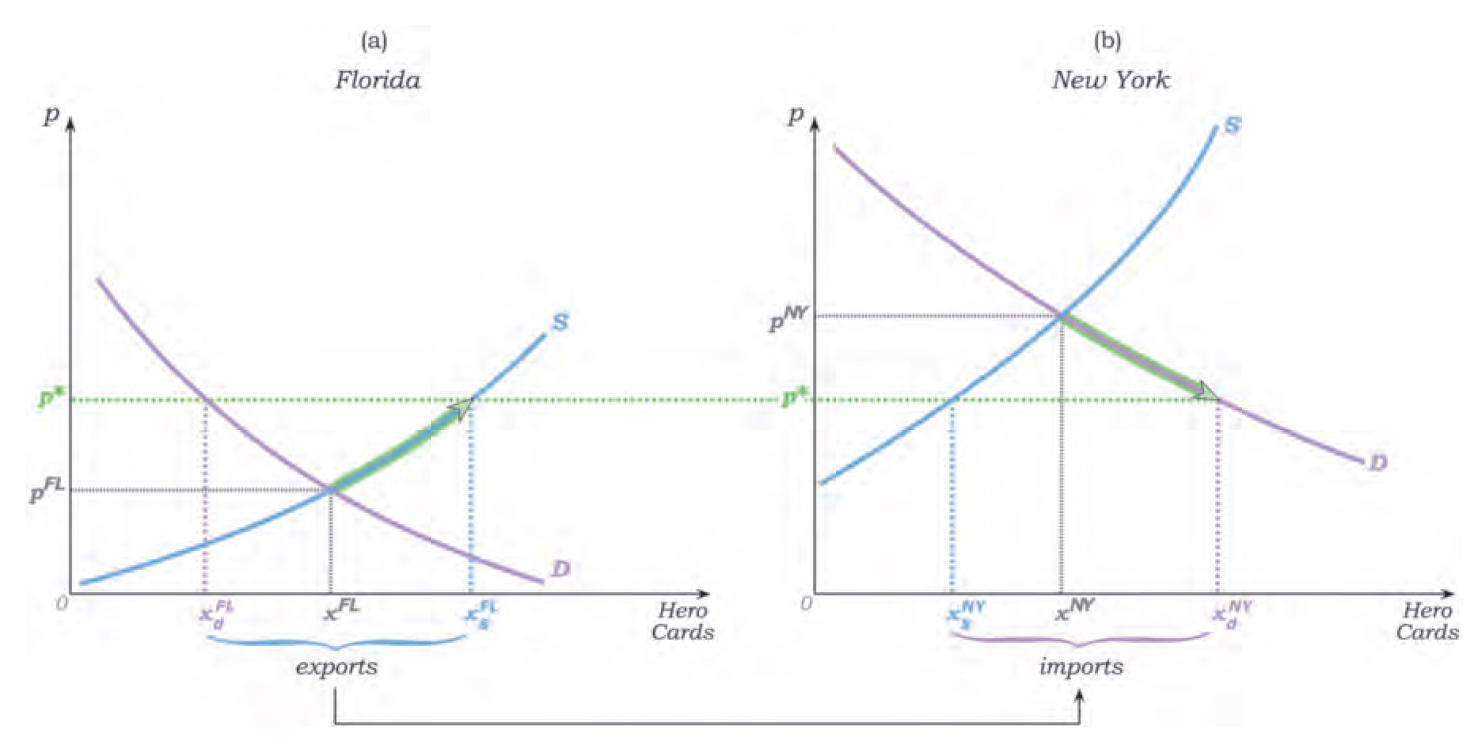
\includegraphics[width=1\textwidth]{20_1} %插入图片,[]中设置图片大小,{}中是图片文件名
	\caption{Equilibrium across 2 Markets} %最终文档中希望显示的图片标题
	\label{Fig.main2} %用于文内引用的标签
\end{figure}

\hspace*{\fill}

出口者与进口者(倒爷)的利润

当我们从“没有贸易”的均衡转向贸易均衡时,出口者和进口者通过低买高卖可以很明显地创造利润。但在模型中两市场达到均衡之后,两市场的出售价格是相同的(倒爷没有利润了),而其实这只是对现实世界的一个近似。现实世界中价格不会完全相等,因为必要的价格差异必须存在弥补商品在两市场运输成本。

出口者和进口者(倒爷)从“没有贸易”均衡转换到贸易均衡的过程中赚取利润。这是一个厂商进入和退出都能够发生的时期,也正是这种任意进入和退出最终使得边际个人利润为零。因而如果进出口行业也是竞争的,从前以得出的结论可知,在新均衡中边际参与者的利润为零。只要利润是正的,额外的经济人都将会进入到进出口行业。

\hspace*{\fill}

跨区域贸易的赢家与输家

出口方厂商获利消费者受损;进口方消费者获利,厂商受损。

\hspace*{\fill}

当贸易被允许时总剩余的变化

\begin{figure}[H] %H为当前位置,!htb为忽略美学标准,htbp为浮动图形
	\centering %图片居中
	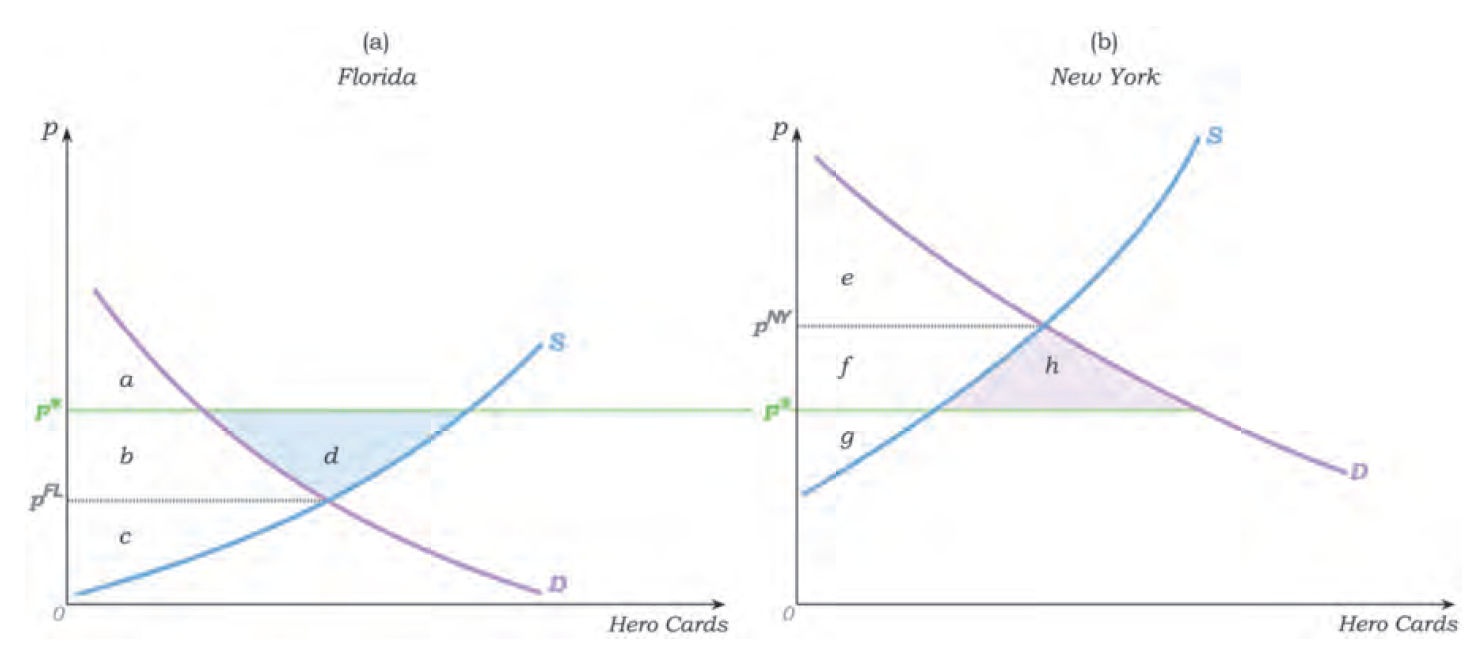
\includegraphics[width=1\textwidth]{20_2} %插入图片,[]中设置图片大小,{}中是图片文件名
	\caption{Changes in Surplus when Trade Is Permitted} %最终文档中希望显示的图片标题
	\label{Fig.main3} %用于文内引用的标签
\end{figure}

两市场贸易开始前的总剩余为:$ a+b+c+e+f+g $,贸易开始后的总剩余为:$ a+b+c+d+e+f+g+h $。

在分析中没有涉及进口者和出口者的剩余内容,因为我们知道,只要进出口行业是竞争的,出口者和进口者的经济利润是零。贸易在总体上使两个区域变得更好,尽管它引起某些经济人受损而其他人受益。但是在贸易中的总剩余增加了,从而导致没有贸易均衡到新均衡的严格Pareto改进。

\hspace*{\fill}

限制贸易与哄抬物价

\subsection{通过关税和进口配额限制贸易}

政府在考虑贸易的限制时有两种选择:通过对贸易商品征税来影响商品的价格,从而限制跨界的商品流,或者直接施加对贸易的数量限制。施加在进口上的税收称为关税(tariff),而限制进口的配额称为进口配额(import quota)。

\hspace*{\fill}

进口上的关税

进口税收的主要影响是限制出口者和进口者的活动。征收关税的本质是施加在这个经济活动上额外的经济成本。

\begin{figure}[H] %H为当前位置,!htb为忽略美学标准,htbp为浮动图形
	\centering %图片居中
	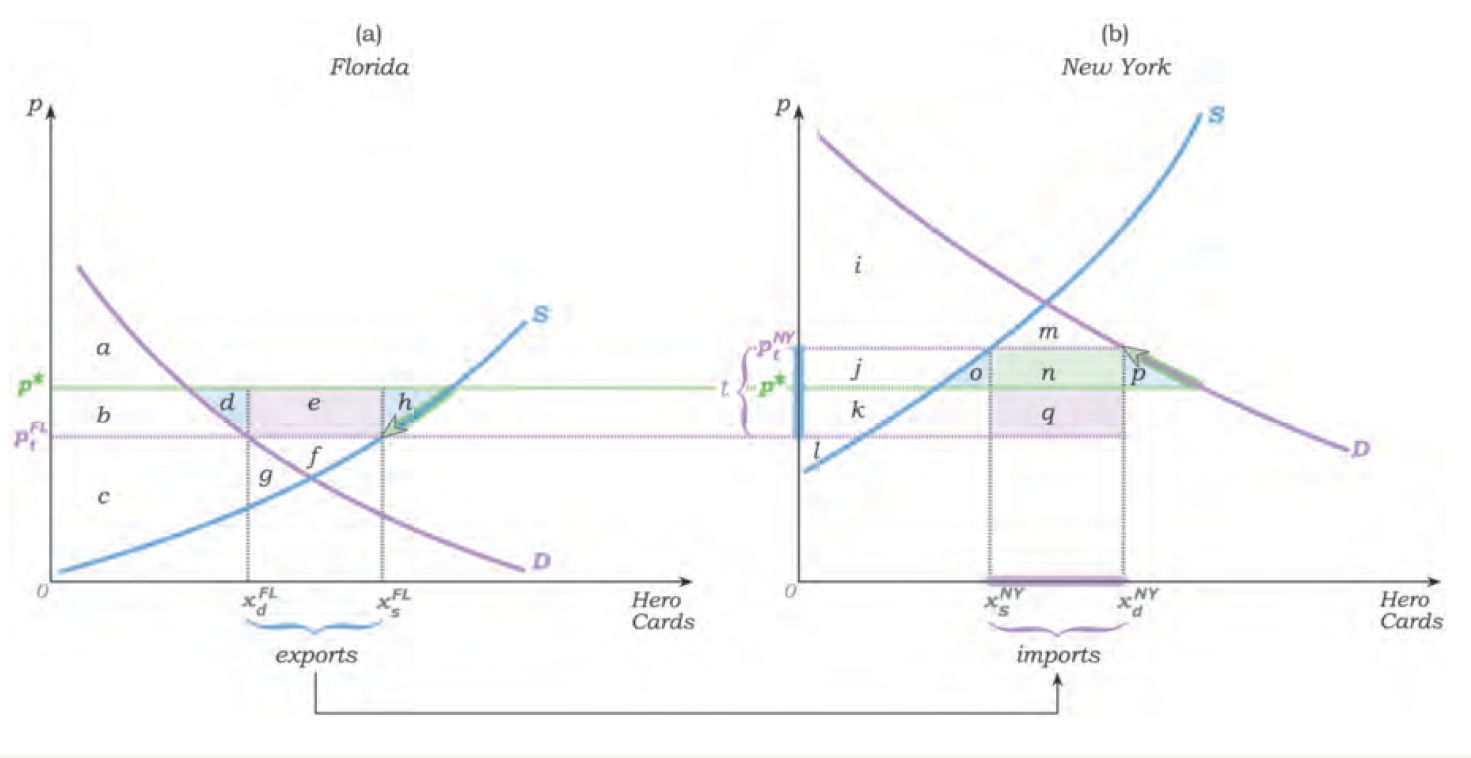
\includegraphics[width=1\textwidth]{20_3} %插入图片,[]中设置图片大小,{}中是图片文件名
	\caption{The Imposition of a Tariff on Hero Cards} %最终文档中希望显示的图片标题
	\label{Fig.main4} %用于文内引用的标签
\end{figure}

当关税t被施加后,出口这和进口者不在创造零利润,因为他们必须为每个进口的商品支付这个税收。因此出口方将减少出口数量,进口方将减少进口数量。这将引起出口价格下降和进口价格上升。这个过程继续直到出口者和进口者再次创造零利润——一旦进/出口价差达到t时这种情况就会发生。在新均衡中,出口的数量是出口地的生产数量与需求数量之差。

由于出口地价格下降,那里的消费者的状况就会变得更好而生产者的状况将会变得更差,对于进口第反之反是。

福利分析:

关税实施前

出口方:消费者剩余为a,生产者剩余为b+c+d+e+f+g+h;

进口方:消费者剩余为i+j+m+n+o+p,生产者剩余为k+l。

关税实施后

出口方:消费者剩余为a+b,生产者剩余为c+g+f,福利损失d+e+h;

进口方:消费者剩余为i+m,生产者剩余为j+k+l,福利损失o+n+p;

进口方政府税收:n+q。

总福利损失:d+h+o+p。

\hspace*{\fill}

把税收的负担传送到其他区域

在一定程度上进口方转移给出口方的关税负担取决于价格弹性。

\begin{figure}[H] %H为当前位置,!htb为忽略美学标准,htbp为浮动图形
	\centering %图片居中
	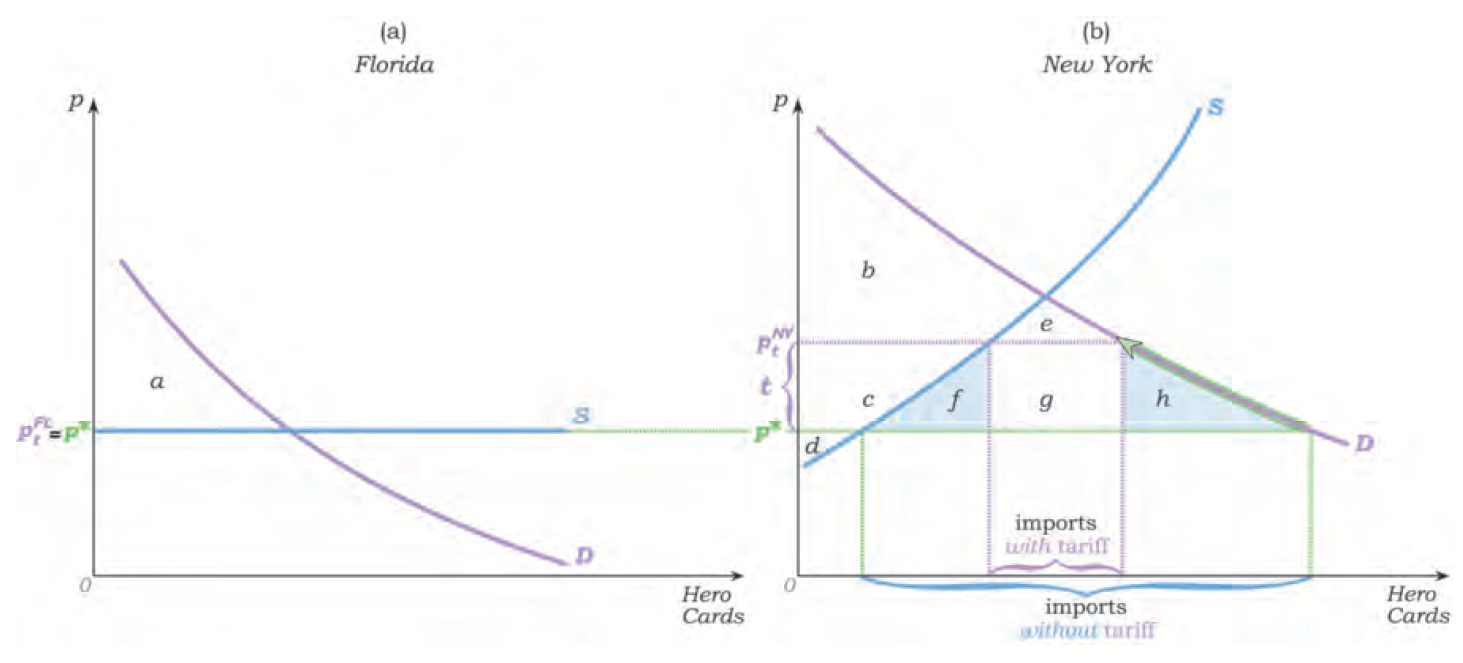
\includegraphics[width=1\textwidth]{20_4} %插入图片,[]中设置图片大小,{}中是图片文件名
	\caption{A Tariff when Supply Is Perfectly Elastic in the Exporting Region} %最终文档中希望显示的图片标题
	\label{Fig.main5} %用于文内引用的标签
\end{figure}

当供给在出口地区是完全弹性时的关税

此时自由贸易意味着在出口地区没有贸易的条件下的价格与在有贸易的条件下的价格相同,最终的结果是进口方承担了所有关税导致的净福利损失。

从而进口市场的供给曲线越有弹性,进口方越有可能从施加的关税中蒙受损失。

\hspace*{\fill}

在区域或国家间的贸易

由于关税带来的进口方所得大于出口方所失,两区域达成一个贸易协定在原则上是可行的。从而,两个区域间协商的贸易协定总能提高两个区域的剩余。

\hspace*{\fill}

进口配额

与关税不一样,进口配额对特定商品有多少可以被进口施加了严格的上限,而关税在名义上允许任意数量的进口。然而,进口配额对价格的影响与关税的影响十分相似。 

\begin{figure}[H] %H为当前位置,!htb为忽略美学标准,htbp为浮动图形
	\centering %图片居中
	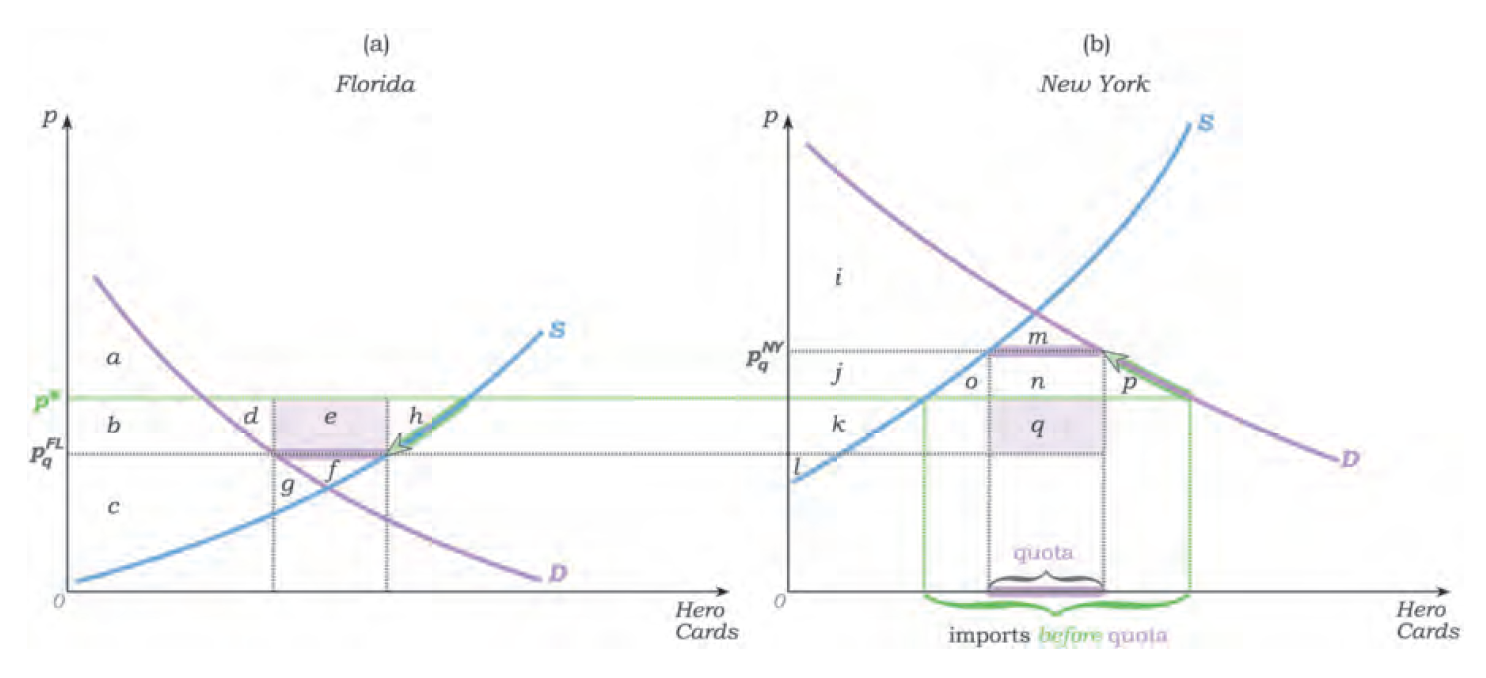
\includegraphics[width=1\textwidth]{20_5} %插入图片,[]中设置图片大小,{}中是图片文件名
	\caption{The Imposition of an Import Quota} %最终文档中希望显示的图片标题
	\label{Fig.main6} %用于文内引用的标签
\end{figure}

在进口配额下,没有税收收入,但此时进出口行业可以获得正的利润n+e。类似地,施加配额所产生的净损失为d+h+o+p。

这种分析并不十分准确,因为我们没有解释如何确定出口者和进口者在以给均衡中获取正的利润。假设每个出口者都想参与这个博弈,这意味着出口者和进口者需要实践额外的努力以在进口配额中获利。这样的努力一定程度上是社会浪费,因此区域e和n的一部分可能实际上是净损失。

\subsection{移民VS外包}

贸易可以发生在劳动力市场中,考虑劳动可以跨区域贸易的两种方式。第一种情况叫“外包”,高工资国家的企业把商品运回并在国内市场出售之前,把一部分劳动密集型的工作送到国外;第二种情形是,不再把生产移到国外以利用其他地方低工资,而是工人们转移到工资较高的地方。自始至终,我们将隐性地假设工人的技能水平/生产力在国家间是相同的。

外包(Outsourcing)

外包生产中地劳动密集型部分到其他国家比国内市场劳动力价格相对便宜地国家,对追求利润最大化地企业是很有吸引力的。

\begin{figure}[H] %H为当前位置,!htb为忽略美学标准,htbp为浮动图形
	\centering %图片居中
	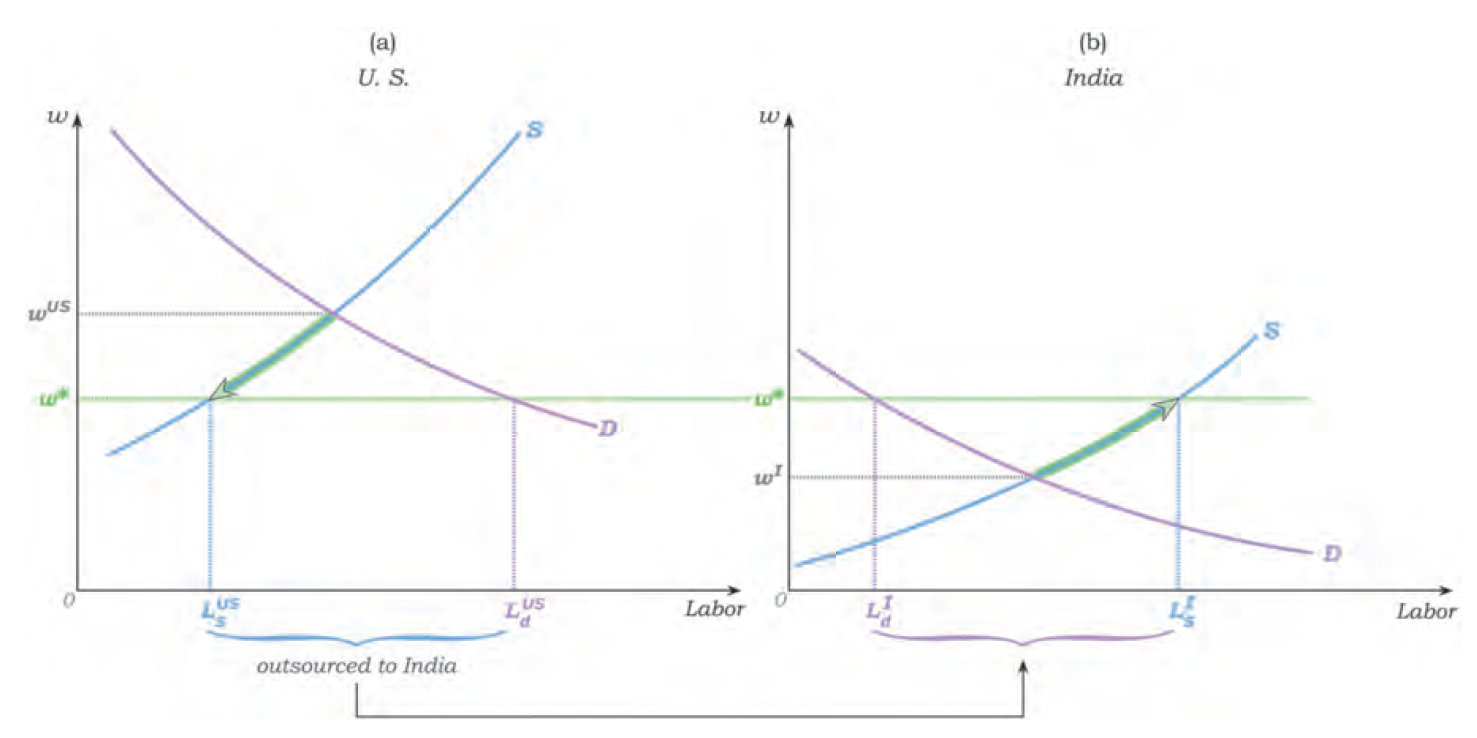
\includegraphics[width=1\textwidth]{20_6} %插入图片,[]中设置图片大小,{}中是图片文件名
	\caption{Outsourcing of Labor-Intensive Jobs from High to Low Wage Countries} %最终文档中希望显示的图片标题
	\label{Fig.main7} %用于文内引用的标签
\end{figure}

现假定外包变为美国生产者地一个经济可行地选择,并进一步假定外包的额外地非劳动成本(如商品地运输)是可忽略的。那么美国生产者的劳动需求将会减少而印度的劳动需求将会增多。这将施加美国劳动市场向下的压力并且施加印度劳动市场工资向上的压力直至均衡。

美国的劳动市场的工人的工资下降了,而印度工人的工资上升了,从而使得美国工人的境况变得更糟糕了而使得印度工人的境况变得更好些。相反,美国生产者经历了更低的劳动成本而印度生产者则面对增加的工资。

\hspace*{\fill}

移民(migration)

\begin{figure}[H] %H为当前位置,!htb为忽略美学标准,htbp为浮动图形
	\centering %图片居中
	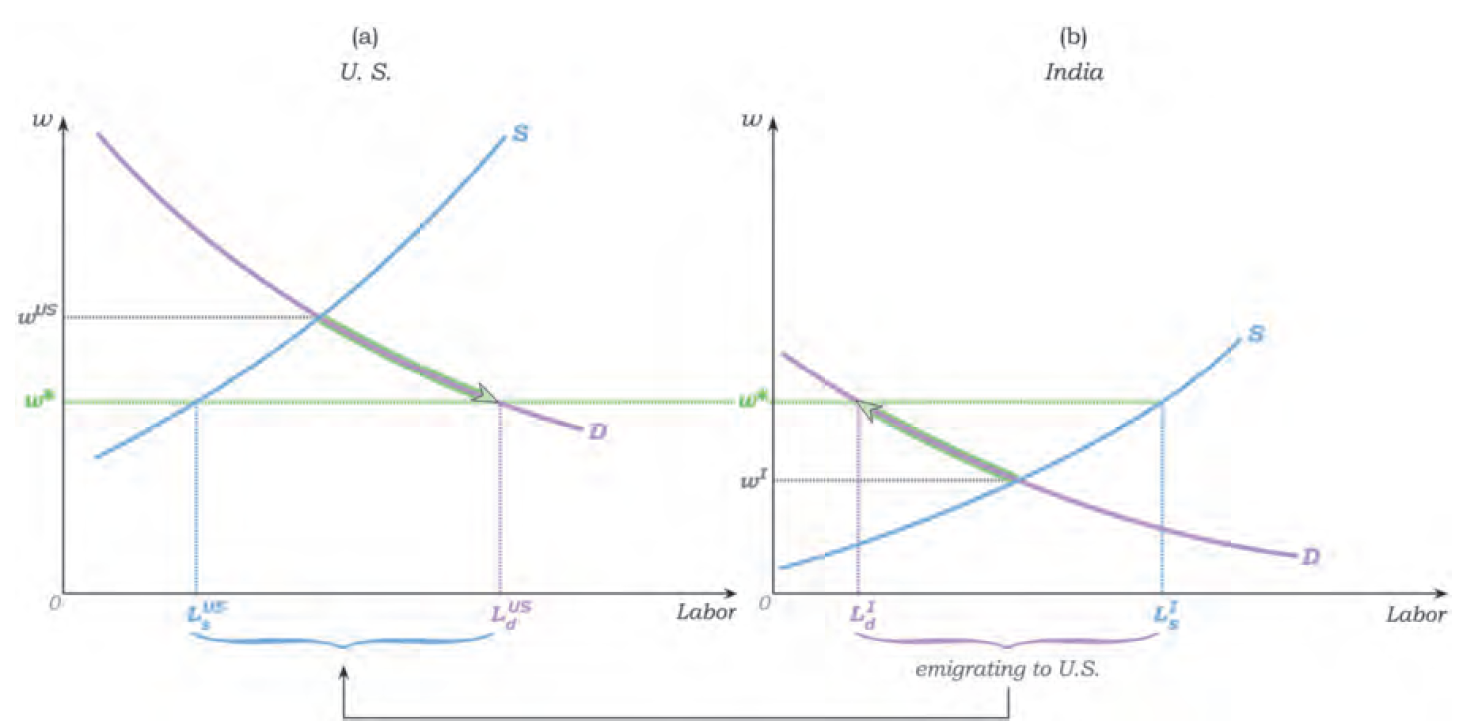
\includegraphics[width=1\textwidth]{20_7} %插入图片,[]中设置图片大小,{}中是图片文件名
	\caption{Migration from High to Low Wage Countries} %最终文档中希望显示的图片标题
	\label{Fig.main8} %用于文内引用的标签
\end{figure}


现在考虑一种发生劳动贸易的可供选择的方式,即劳动而不是生产从一个国家转移到另一个国家。由于生产不是从一个国家转移到另一个国家,劳动需求在这两个国家将会保持不变,但是劳动供给曲线会随着印度为获得较高的工资而移民到美国的劳动的移动而移动。

类似地,新工资$ w^* $处印度劳动市场供给曲线与需求曲线的劳动的差表示印度工人在美国所提供的劳动。

美国工资向下的压力和印度工资向上的压力在外包下沿着供给曲线产生而移民时沿着需求曲线产生。这是因为当企业移动工作时,市场工资的压力产生于两个国家中劳动需求曲线的移动,而当工人在两给国家间自身移动时,该压力产生于两给国家中劳动供给曲线的移动。然而,一旦达到新均衡后最终的效果将完全相同。

\hspace*{\fill}

移动商品还是移动人

外包要求商品移动,而移民要求人移动。外包要求交易商品的较低障碍以使得高工资国家的公司能将生产部门移到低工资国家,并接着把商品运输回需求不成比例的高工资国家。另一方面,移民要求较低的劳动移动障碍以使得工人能够移动到工资较高的地方。二者对工资有相同的终极影响的预测,这是因为两种机制都提供了整合两个劳动力市场的方式。在两种情形下,高工资国家的人在本质上从低工资国家雇佣工人来为他们生产产品。

话虽如此,但事实上贸易和移民尽管增加了所有国家的总剩余,但也在国家间带来了赢家和输家。

\subsection{跨时贸易}

“跨时贸易”与“跨空间贸易”不同——跨时贸易能导致较少的稳定性。跨空间贸易和跨时贸易的重要区别是前者发生在相对确定的环境中而后者发生在相对不确定的环境中。

\begin{figure}[H] %H为当前位置,!htb为忽略美学标准,htbp为浮动图形
	\centering %图片居中
	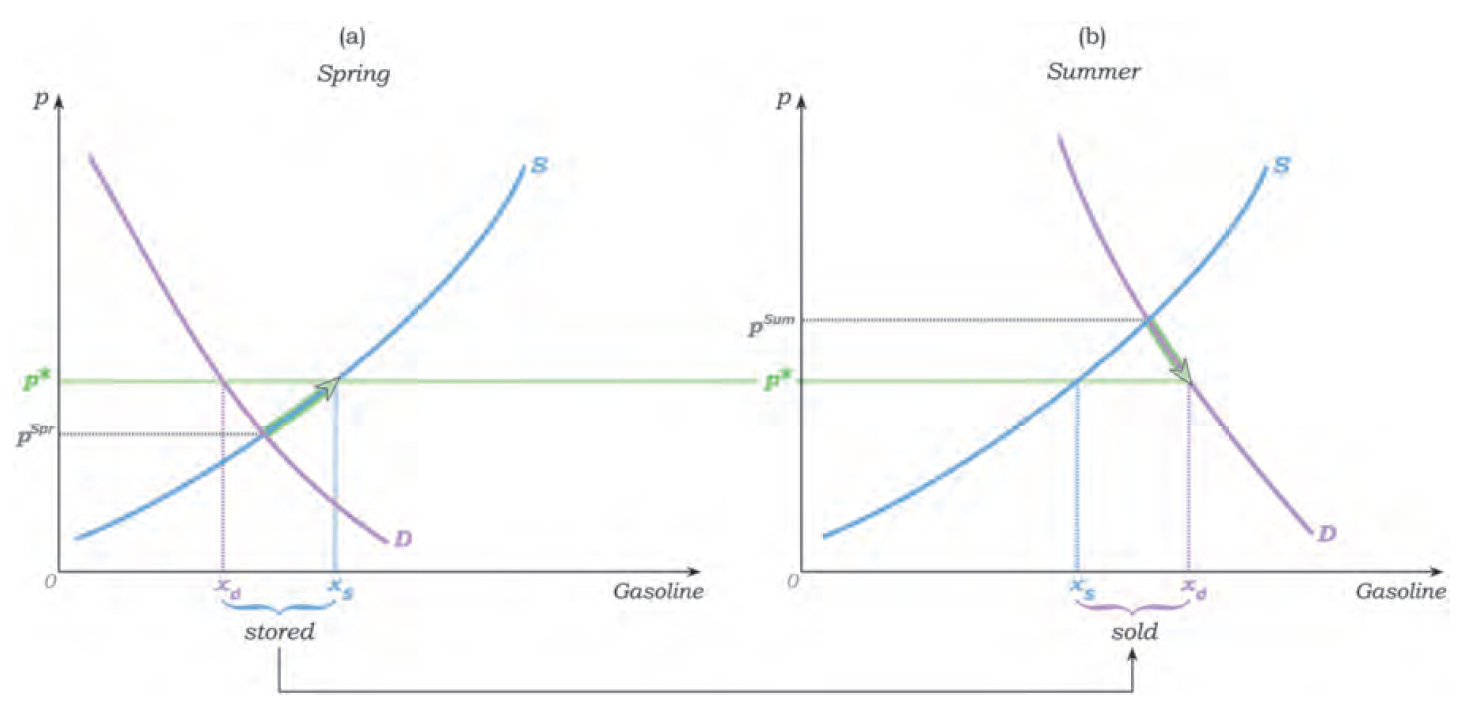
\includegraphics[width=1\textwidth]{20_8} %插入图片,[]中设置图片大小,{}中是图片文件名
	\caption{Speculation and the Price of Gasoline} %最终文档中希望显示的图片标题
	\label{Fig.main9} %用于文内引用的标签
\end{figure}

假设由于供需春季的汽油价格较低以及在没有跨时贸易时夏季的汽油价格较高。但若跨时交易是可以的,假定储存成本可以忽略。投机者将在春季购买低价汽油并在夏季卖出,导致了春天增加的需求和在夏季增加的供给,这将引起在春季汽油向上的压力以及在夏季汽油价格向下的压力。







	
\end{document}